Вторым экспериментом было проведение сравнения результатом для различных ReID моделей. Благодаря этому, можно будет понять, насколько использование более требовательных моделей оправдано. 

В ходе эксперимента, для каждой сети детектора и размера изображения из прошлого пункта был проведен анализ точности работы отдельных ReID моделей на наборе данных MOT17. Полученные результаты можно увидеть на рисунках \ref{fig:yolo_reid_ByteTrack}-\ref{fig:yolo_reid_ImprAssOC}. Отдельно стоит отметить, что на рисунках \ref{fig:yolo_reid_ByteTrack}-\ref{fig:yolo_reid_OC-SORT} нет влияния выбора, так как реализации алгоритмом ByteTrack и OC-SORT не используют ReID модели, а основываются на метрике IoU.

Полученные графики явно показывают, что только самая маленькая ReID модель OSNet x0.25 дает стабильно более низкий результат. При этом все остальные модели дают абсолютно схожие показатели с минимальными улучшениями относительно друг друга.
\begin{figure}[ht]
    \centering
    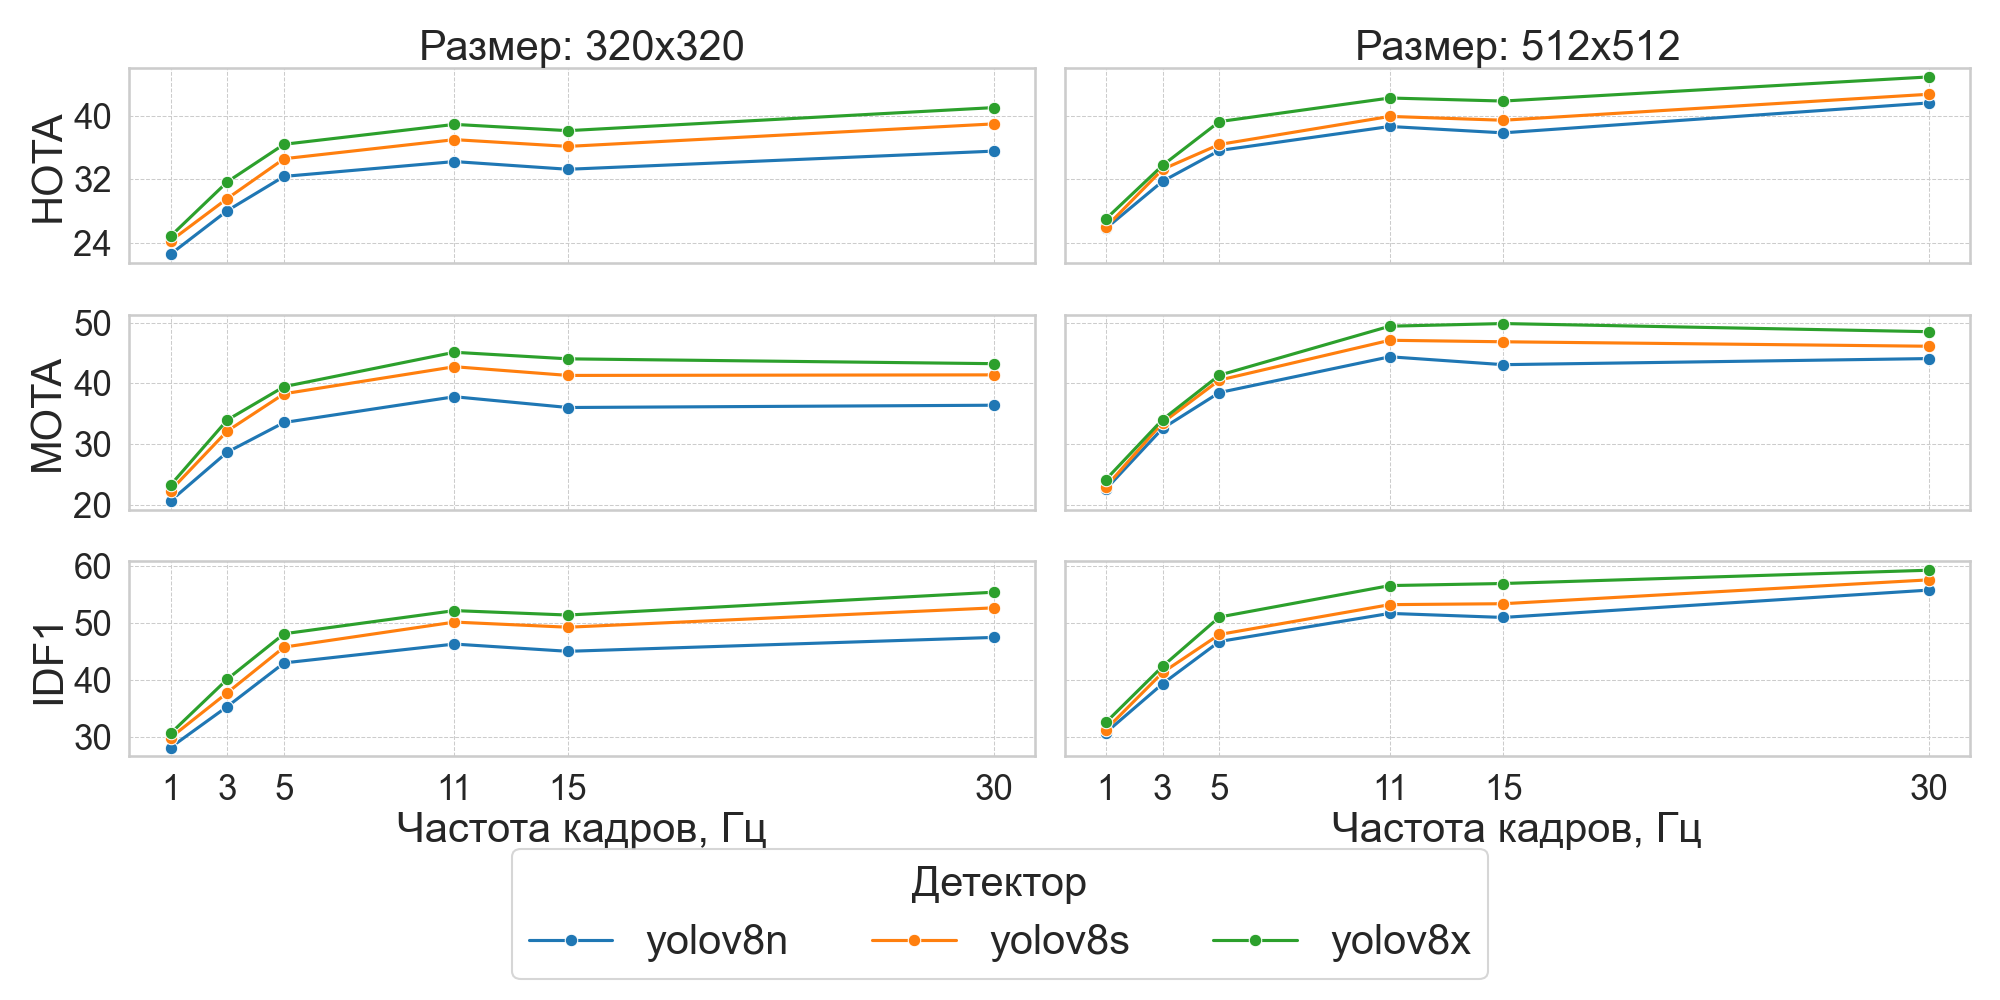
\includegraphics[width=1\textwidth]{plots/yolo_size_and_reid_vs_metric/ByteTrack.png}
    \caption{График зависимости метрик HOTA, MOTA и IDF1 от ReID модели для алгоритма ByteTrack}
    \label{fig:yolo_reid_ByteTrack}
\end{figure}

\begin{figure}[ht]
    \centering
    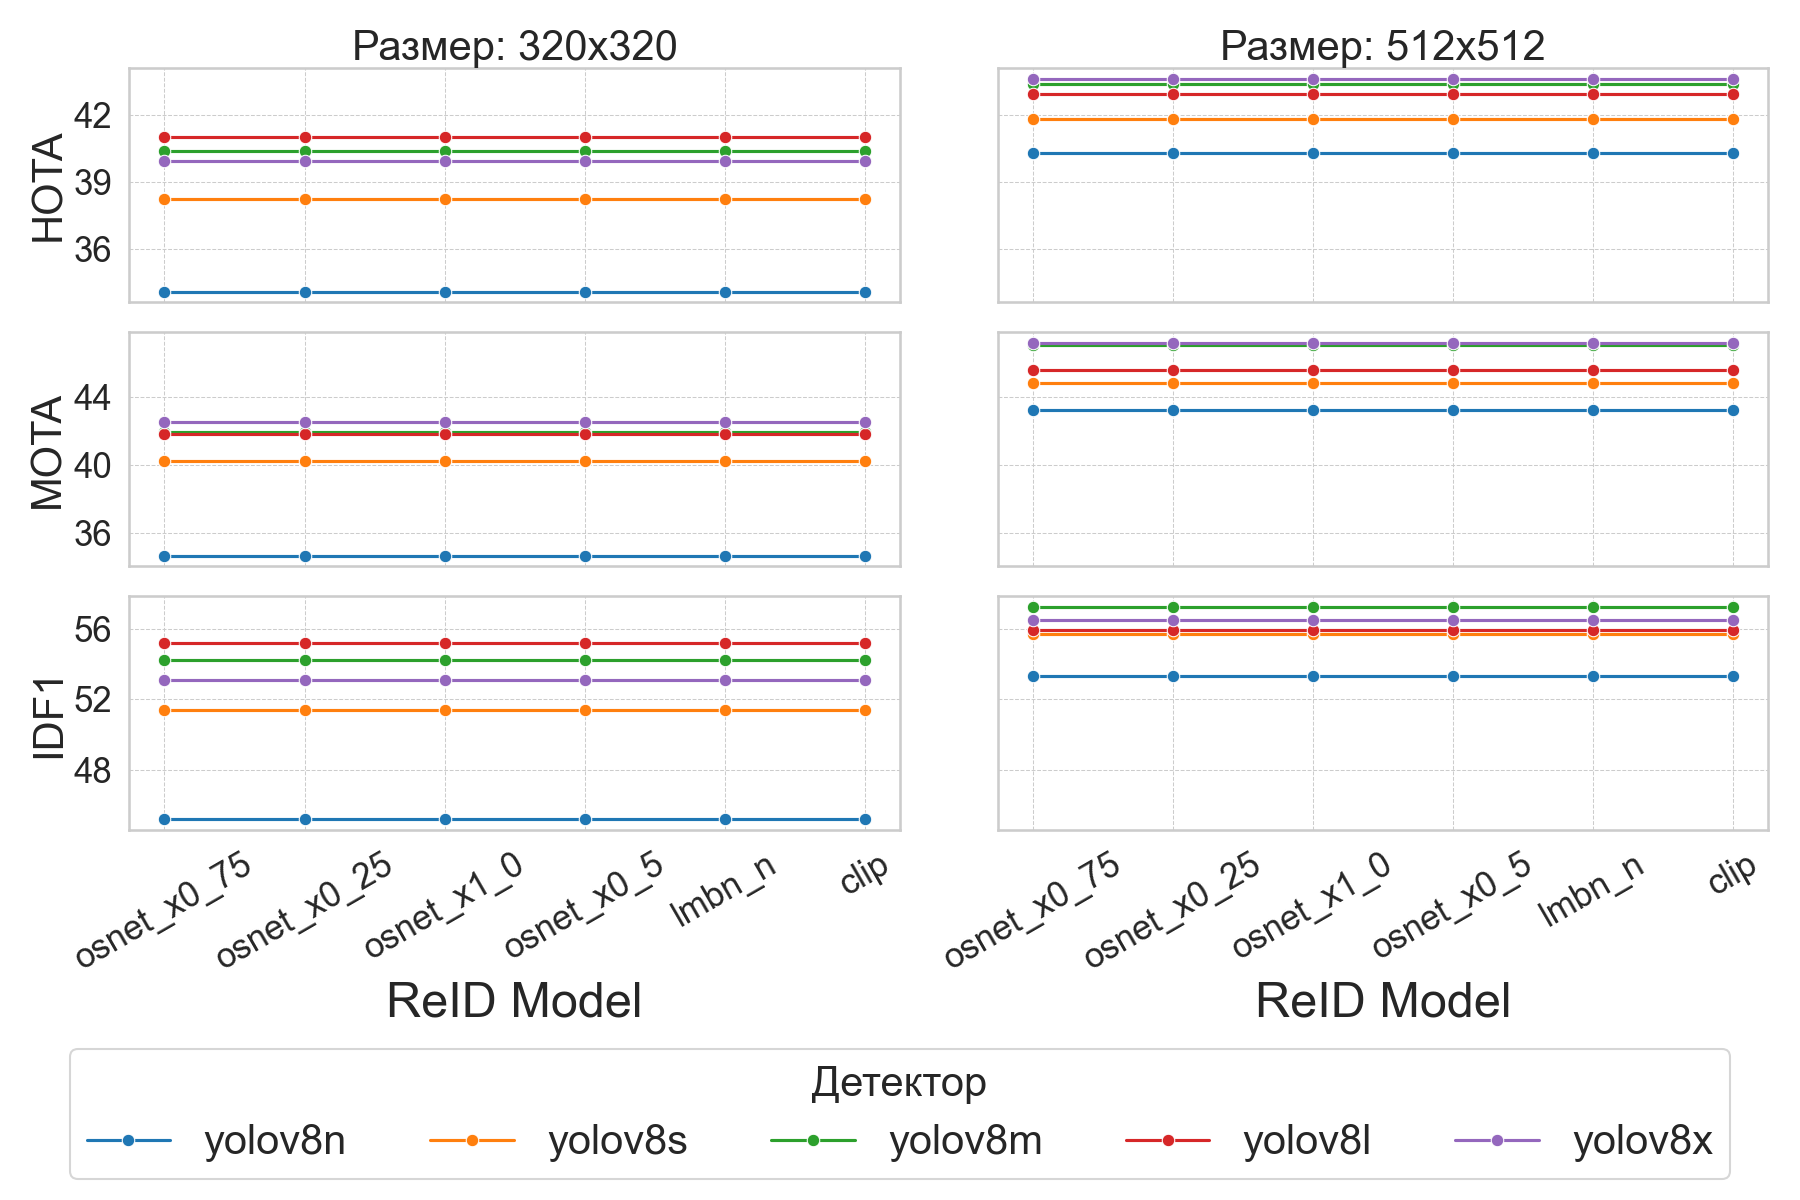
\includegraphics[width=1\textwidth]{plots/yolo_size_and_reid_vs_metric/OC-SORT.png}
    \caption{График зависимости метрик HOTA, MOTA и IDF1 от ReID модели для алгоритма OC-SORT}
    \label{fig:yolo_reid_OC-SORT}
\end{figure}

\begin{figure}[ht]
    \centering
    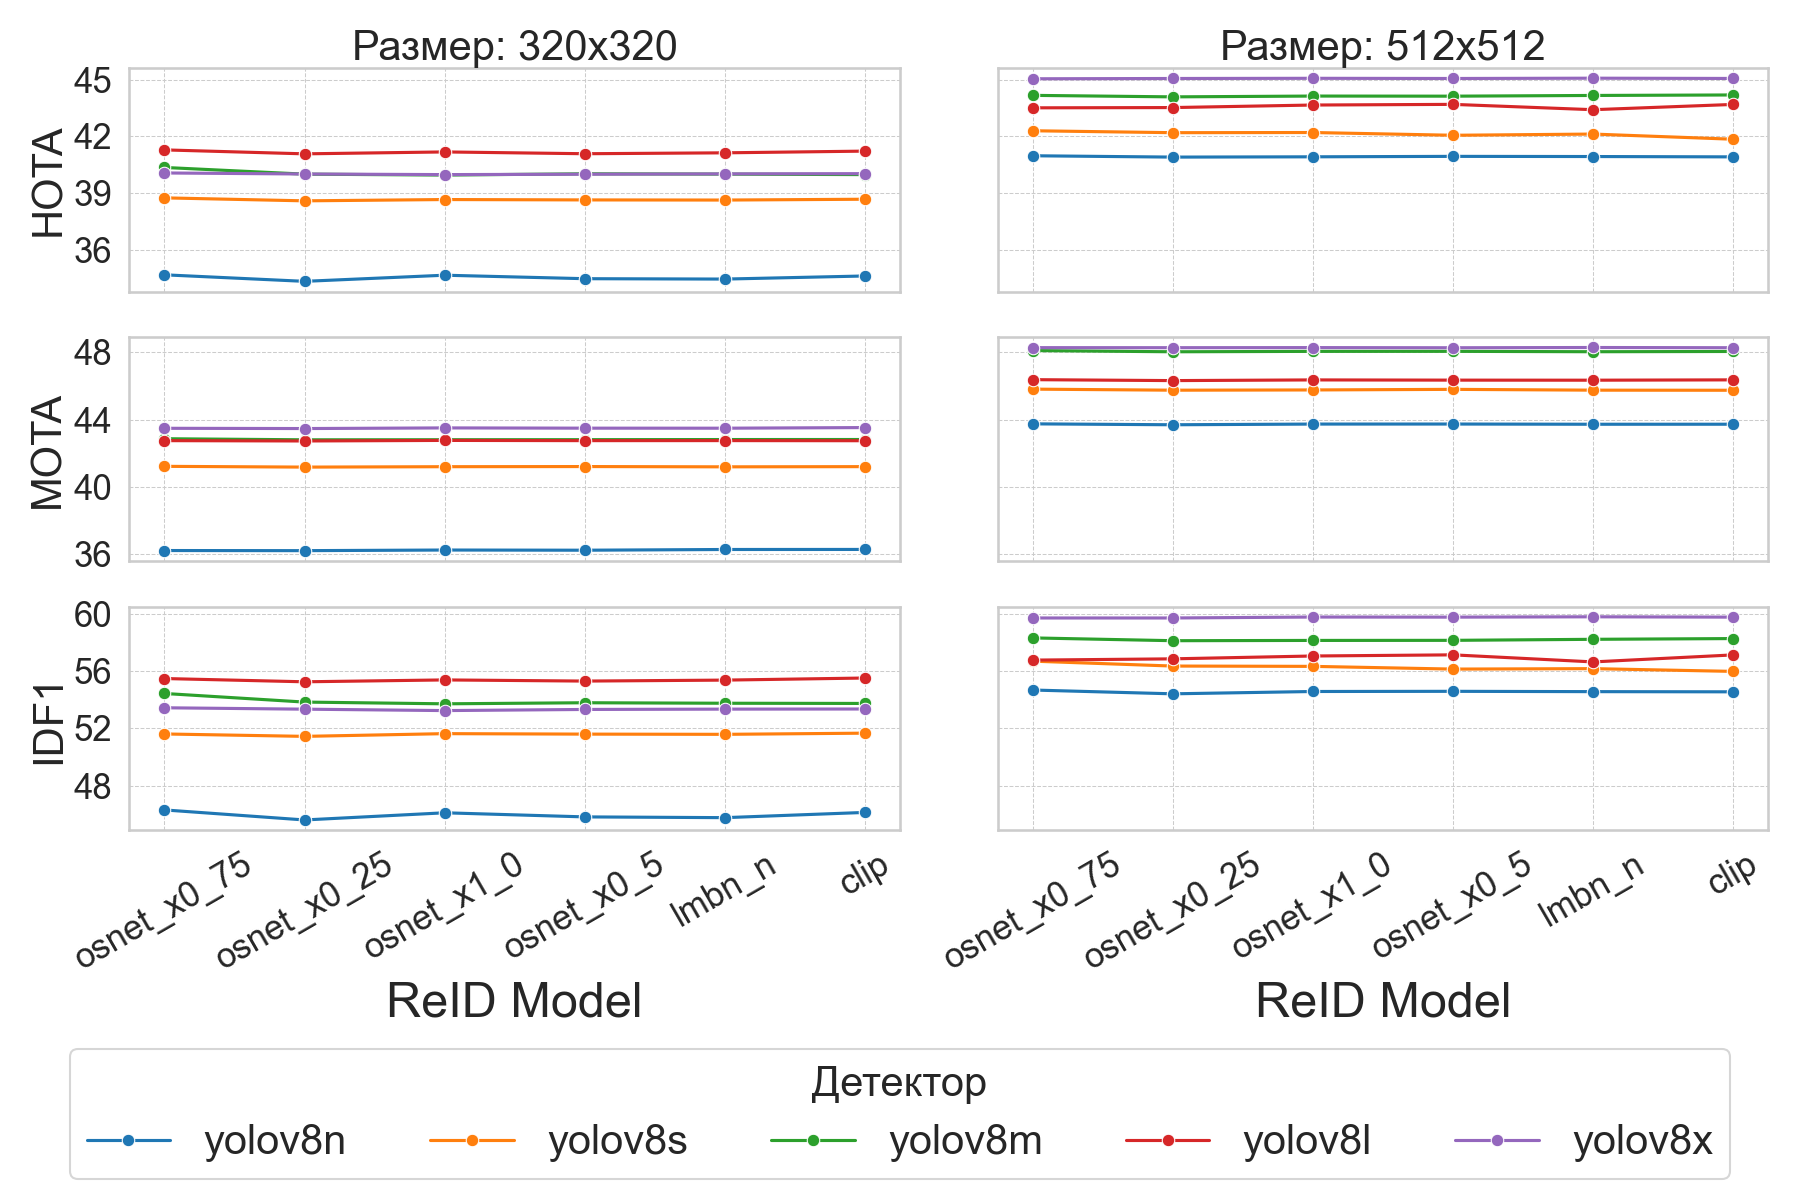
\includegraphics[width=1\textwidth]{plots/yolo_size_and_reid_vs_metric/Deep OC-SORT.png}
    \caption{График зависимости метрик HOTA, MOTA и IDF1 от ReID модели для алгоритма Deep OC-SORT}
    \label{fig:yolo_reid_Deep OC-SORT}
\end{figure}

\begin{figure}[ht]
    \centering
    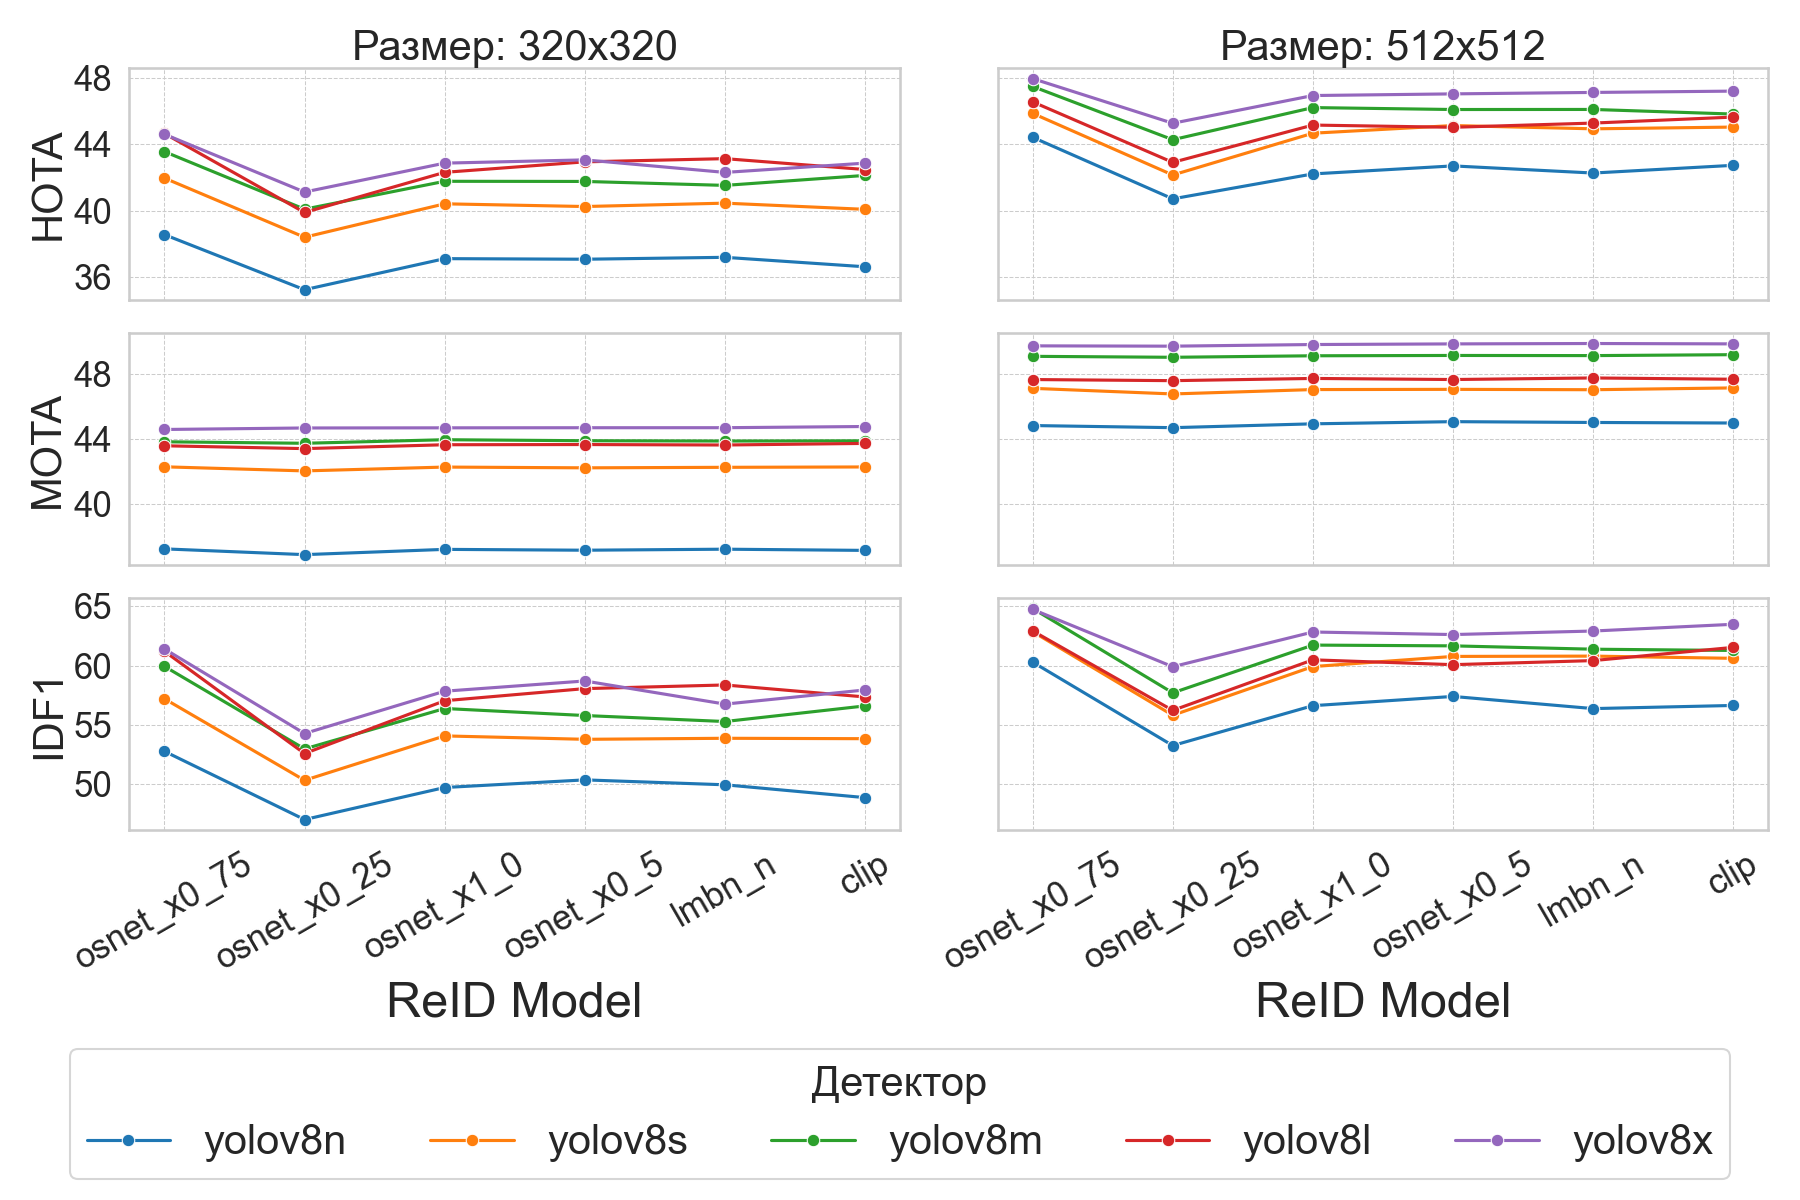
\includegraphics[width=1\textwidth]{plots/yolo_size_and_reid_vs_metric/StrongSORT.png}
    \caption{График зависимости метрик HOTA, MOTA и IDF1 от ReID модели для алгоритма StrongSORT}
    \label{fig:yolo_reid_StrongSORT}
\end{figure}

\begin{figure}[ht]
    \centering
    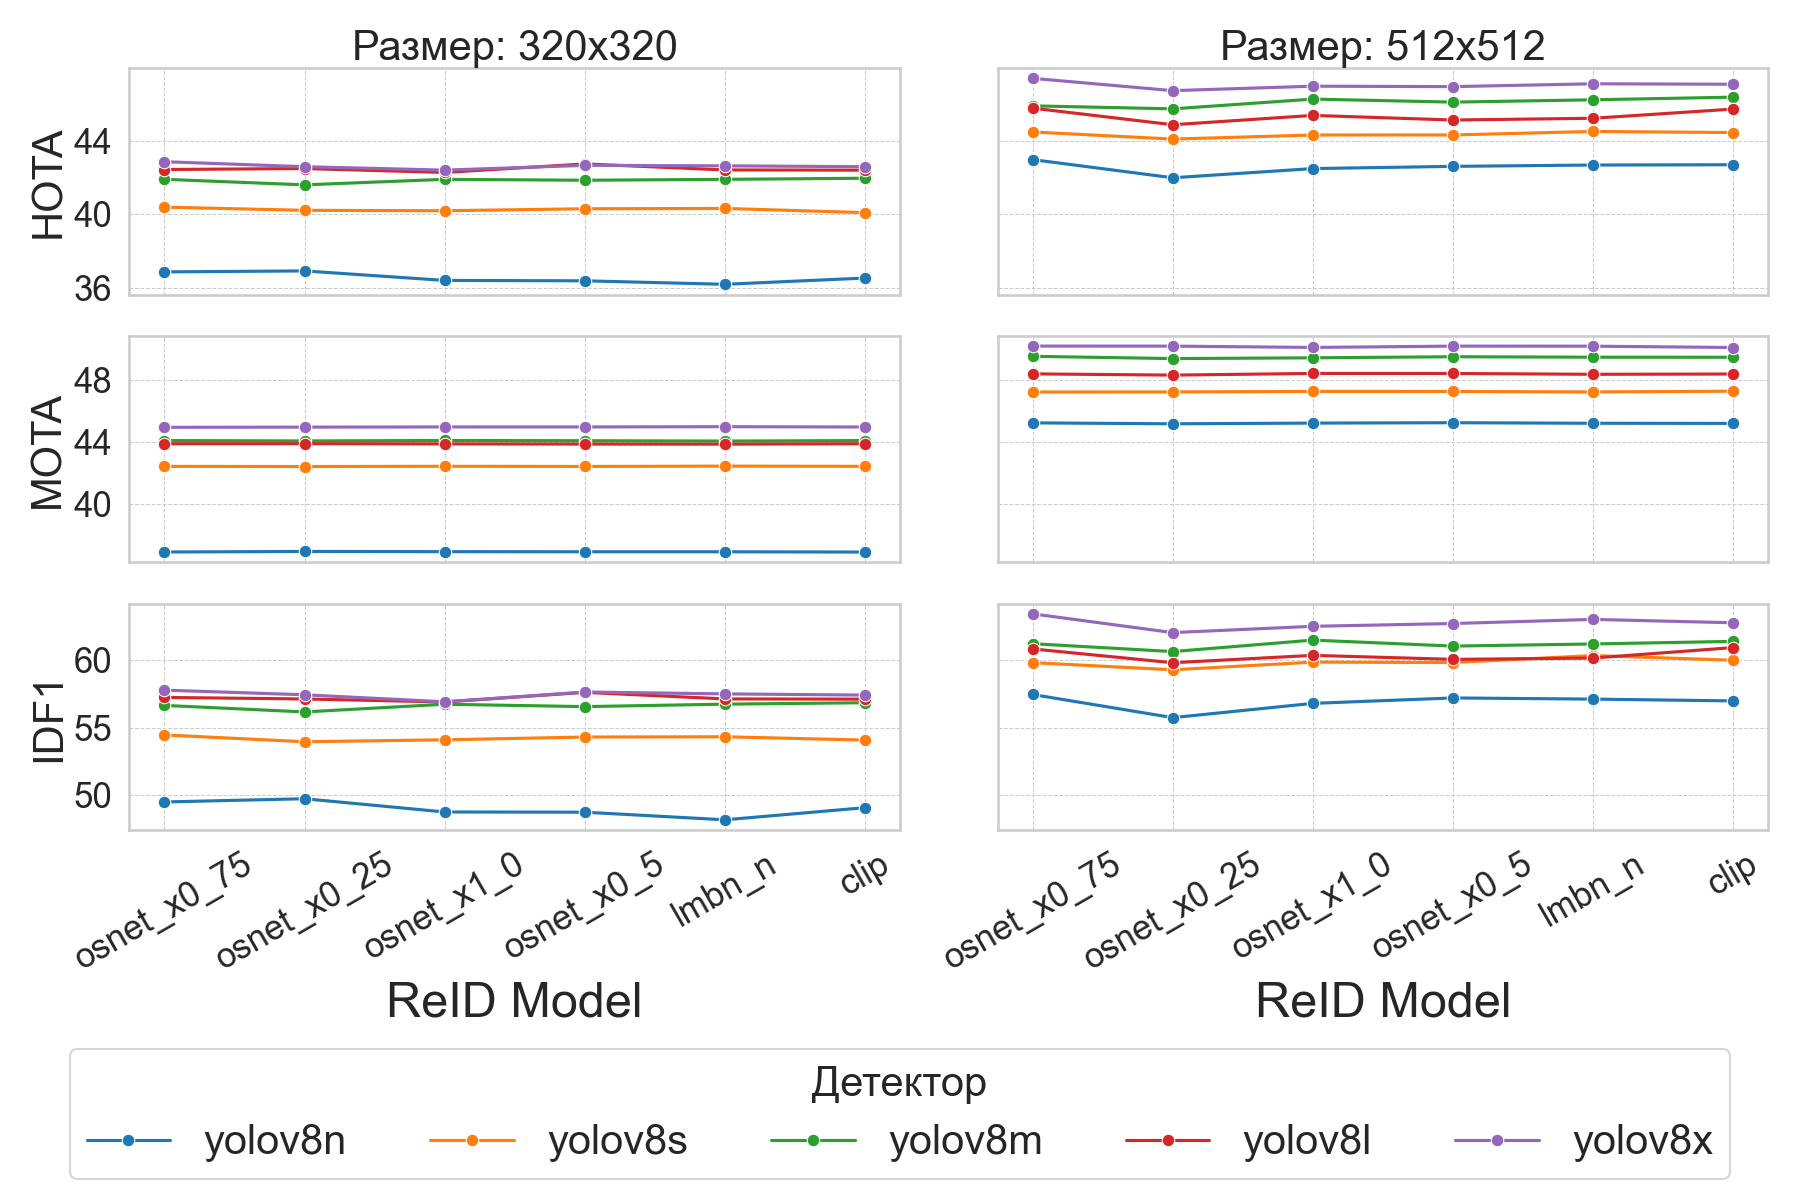
\includegraphics[width=1\textwidth]{plots/yolo_size_and_reid_vs_metric/BoT-SORT.png}
    \caption{График зависимости метрик HOTA, MOTA и IDF1 от ReID модели для алгоритма BoT-SORT}
    \label{fig:yolo_reid_BoT-SORT}
\end{figure}

\begin{figure}[ht]
    \centering
    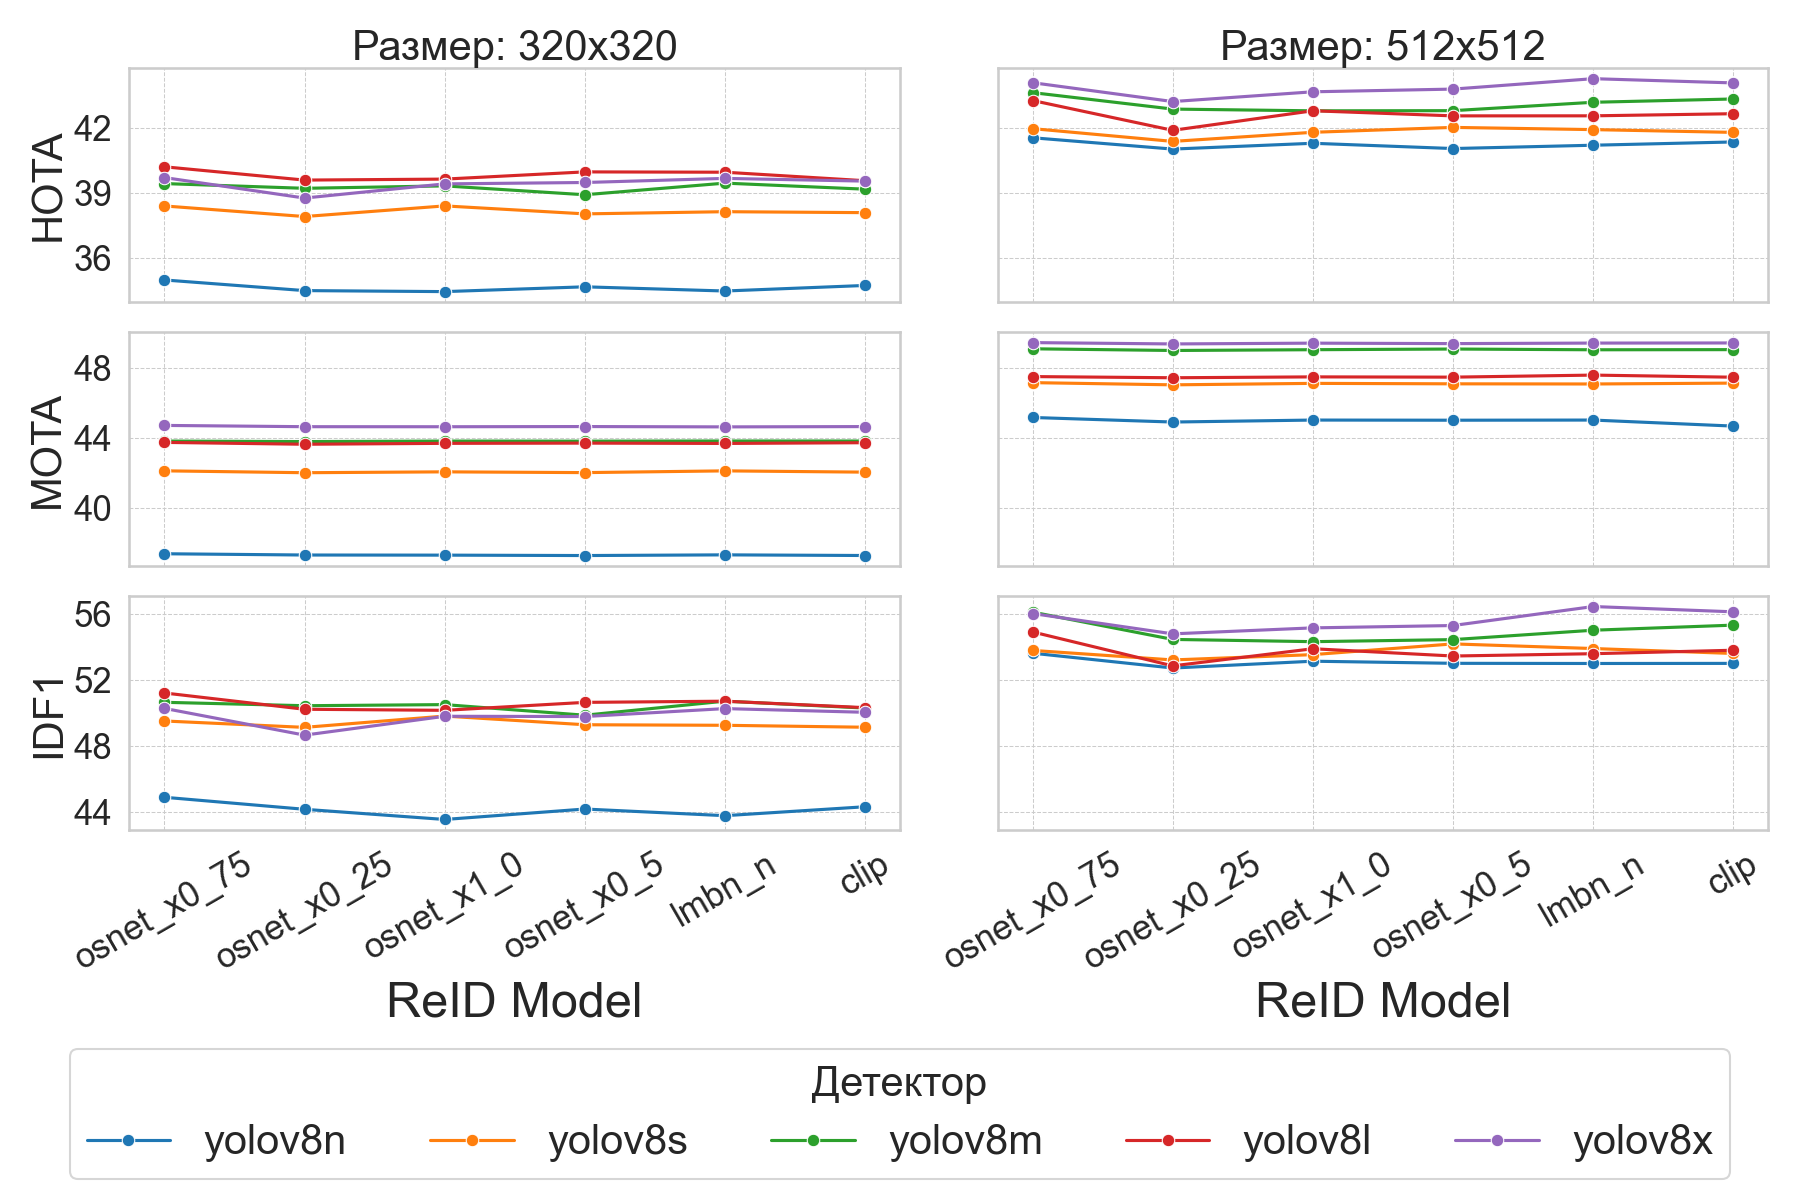
\includegraphics[width=1\textwidth]{plots/yolo_size_and_reid_vs_metric/ImprAssOC.png}
    \caption{График зависимости метрик HOTA, MOTA и IDF1 от ReID модели для алгоритма ImprAssOC}
    \label{fig:yolo_reid_ImprAssOC}
\end{figure}
\FloatBarrier

% TODO: можно добавить сравнения на низких фпс табличку, там вроде то же самое, но для объема